\documentclass[pdf,usenames,dvipsnames,tikz]{beamer}%usenames and dvipsnames are for colours.
%TODO: Maybe use aspectratio=169
\mode<presentation>{}
\usetheme{Madrid}
\usecolortheme{seahorse}

\usepackage{amsmath}
\usepackage{siunitx}
\usepackage{enumerate}

%Localisation
\usepackage{csquotes} %Context sensitive quotes: recommended by babel polyglossia
\usepackage[british]{babel}

\usepackage{tikz}
\usetikzlibrary{positioning,arrows}

\usepackage{graphicx}
\graphicspath{ {./images/} {./biol375-report/figures/} }

\usepackage{hyperref}
\hypersetup{
	colorlinks=true,
	urlcolor=blue,
}
\urlstyle{same} %URLs are set in the font of the surrounding text

\usepackage{booktabs}

%Generic math commands
\newcommand\norm[1]{\left\lVert#1\right\rVert}
\newcommand\abs[1]{\left\lvert#1\right\rvert}
\renewcommand\d{\mathrm{d}}
\newcommand\D[1]{\mathop{\d #1}}
\newcommand\e{\mathrm{e}}
\newcommand\Imat{\mathrm{I}}
%Need this so that mathrm isn't serif, 'cause the rest of the beamer stuff is sans.
\renewcommand\mathrm[1]{\text{#1}}

\usepackage[backend=biber,style=verbose]{biblatex}
\addbibresource{references.bib}
\setbeamertemplate{navigation symbols}{}

%Remove numbers from footcite.
\let\innerfootcite\footcite
\renewcommand\footcite[1]{%
	\begingroup
	\renewcommand\thefootnote{}\innerfootcite{#1}%
	\addtocounter{footnote}{-1}%
	\endgroup
}

\title{The Hausdorff Metric}
\subtitle{A Dissimilarity Metric for Partially Ranked Data}
\author{Christopher Brown}
\date{}

\begin{document}

%Title frame
\begin{frame}
	\titlepage
\end{frame}

\begin{frame}{The Inspiration}
	Coded abundance for the\\Semi-Quantitative Macroinvertebrate Community Index\footcite{sqmci}:
	
	\medskip
	
	\begin{tabular}{ll}
		\toprule
		Coded Abundance & Number of Individuals\\
		\midrule
		0 & 0\\
		1 & 1--4\\
		5 & 5--19\\
		20 & 20--99\\
		100 & 100--499\\
		500 & $\geq500$\\
		\bottomrule
	\end{tabular}
\end{frame}

\begin{frame}{Another Example}
	Braun-Blanquet cover-abundance scale\footcite{braun-blanquet}:
	
	\medskip
	
	\begin{tabular}{lll}
		\toprule
		Braun-Blanquet Score & Cover & Number of Individuals\\
		\midrule
		+ & $<\SI{5}{\percent}$ & Few\\
		1 & $<\SI{5}{\percent}$ & Many\\
		2 & \SIrange{5}{25}{\percent}\\
		3 & \SIrange{25}{50}{\percent}\\
		4 & \SIrange{50}{75}{\percent}\\
		5 & \SIrange{75}{100}{\percent}\\
		\bottomrule
	\end{tabular}
\end{frame}

\begin{frame}{Ranking}
	\centering
	\begin{tabular}{lcccc}
		\toprule
		Species & A  & B  & C  & D \\
		Score   & 1  & 20 & 0  & 5 \\
		\bottomrule
	\end{tabular}
	
	\bigskip\bigskip
	
	
\begin{tikzpicture}[node distance=0.2cm]
		\node (a1)               {C};
		\node (a2) [right=of a1] {A};
		\node (a3) [right=of a2] {D};
		\node (a4) [right=of a3] {B};
		\node (a)  [left=of  a1] {Ranking:};
	\end{tikzpicture}
\end{frame}

\begin{frame}{Edit Distance: Kendall's Tau}
	\centering
	
	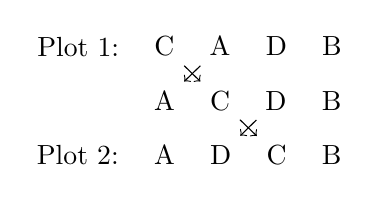
\begin{tikzpicture}[node distance=0.2cm]
		\node (a1)               {C};
		\node (a2) [right=of a1] {A};
		\node (a3) [right=of a2] {D};
		\node (a4) [right=of a3] {B};
		\node (a)  [left=of  a1] {Plot 1:};
		
		\node (b1) [below=of a1] {A};
		\node (b2) [right=of b1] {C};
		\node (b3) [right=of b2] {D};
		\node (b4) [right=of b3] {B};
		
		\node (c1) [below=of b1] {A};
		\node (c2) [right=of c1] {D};
		\node (c3) [right=of c2] {C};
		\node (c4) [right=of c3] {B};
		\node (c)  [left=of  c1] {Plot 2:};
		
		\draw [->] (a1) to (b2);
		\draw [->] (a2) to (b1);
		
		\draw [->] (b2) to (c3);
		\draw [->] (b3) to (c2);
	\end{tikzpicture}
	
	\bigskip
	
	Dissimilarity of 2
\end{frame}

\begin{frame}{Partial Ranking}
	\centering
	\begin{tabular}{lcccc}
		\toprule
		Species & A  & B  & C  & D \\
		Score   & 1  & 5  & 0  & 5 \\
		\bottomrule
	\end{tabular}
	
	\bigskip\bigskip
	
	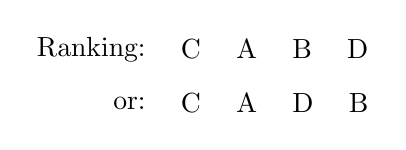
\begin{tikzpicture}[node distance=0.2cm]
		\node (a1)               {C};
		\node (a2) [right=of a1] {A};
		\node (a3) [right=of a2] {B};
		\node (a4) [right=of a3] {D};
		\node (a)  [left=of  a1] {Ranking:};
		
		\node (b1) [below=of a1] {C};
		\node (b2) [right=of b1] {A};
		\node (b3) [right=of b2] {D};
		\node (b4) [right=of b3] {B};
		\node (b)  [left=of  b1] {or:};
	\end{tikzpicture}
\end{frame}

\begin{frame}{Hausdorff Distance}
	\centering
	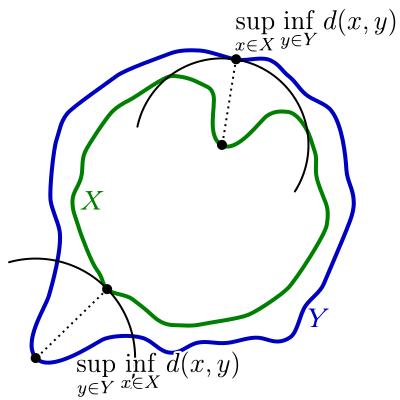
\includegraphics[width=0.6\textwidth]{hausdorff}
\end{frame}

\begin{frame}{Hausdorff Edit Distance}
	\centering
	\begin{tabular}{cc}
		\begin{tabular}{lcccc}
			\toprule
			Species & A  & B  & C  & D \\
			Score   & 1  & 5  & 0  & 5 \\
			\bottomrule
		\end{tabular}
		
		\bigskip\bigskip
		
		&
		
		\begin{tabular}{lcccc}
			\toprule
			Species & A  & B  & C  & D \\
			Score   & 5  & 1  & 0  & 5 \\
			\bottomrule
		\end{tabular}
		
		\bigskip\bigskip
		
		\\
		
		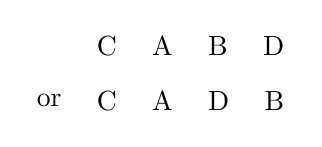
\begin{tikzpicture}[node distance=0.2cm]
			\node (a1)               {C};
			\node (a2) [right=of a1] {A};
			\node (a3) [right=of a2] {B};
			\node (a4) [right=of a3] {D};
			
			\node (b1) [below=of a1] {C};
			\node (b2) [right=of b1] {A};
			\node (b3) [right=of b2] {D};
			\node (b4) [right=of b3] {B};
			\node (b)  [left=of  b1] {or};
		\end{tikzpicture}
		
		&
		
		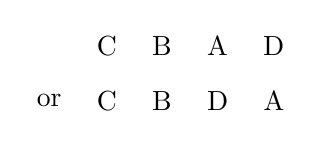
\begin{tikzpicture}[node distance=0.2cm]
			\node (a1)               {C};
			\node (a2) [right=of a1] {B};
			\node (a3) [right=of a2] {A};
			\node (a4) [right=of a3] {D};
			
			\node (b1) [below=of a1] {C};
			\node (b2) [right=of b1] {B};
			\node (b3) [right=of b2] {D};
			\node (b4) [right=of b3] {A};
			\node (b)  [left=of  b1] {or};
		\end{tikzpicture}
	\end{tabular}
	\footcite{critchlow}
\end{frame}

\begin{frame}{Results}
	\centering
	\includegraphics[width=0.6\textwidth]{site-ordination}
\end{frame}

\begin{frame}
	\printbibliography
\end{frame}

\end{document}
